%% ==================
\chapter{Results}
\label{ch:results}
%% ==================
%
%My results:

\section{Recreating previous results}
%	-Only 3 original components
%		-Spherical excess
%		-very bad chi2 in disk and bubbles

Introduce the weniger plots here (or in the state of the research?) to show excess in GC.
\begin{figure}
  \centering
  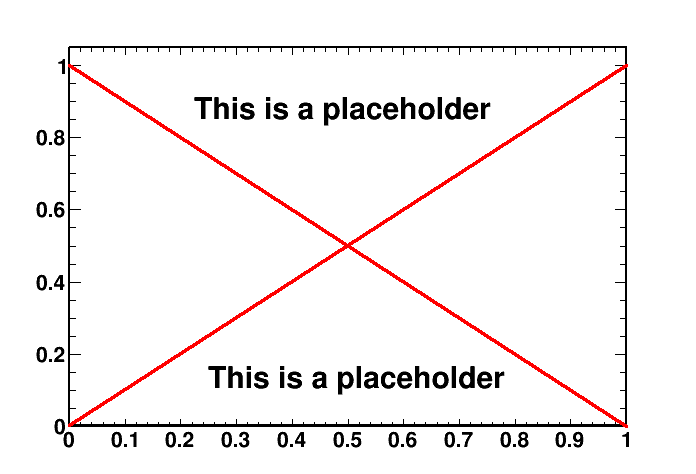
\includegraphics[width=.9\linewidth]{pic/dummy.png}
  \caption{Some weniger plots to show the GC excess}
  \label{fig:weniger_plot}
\end{figure}



\begin{figure}
  \centering
  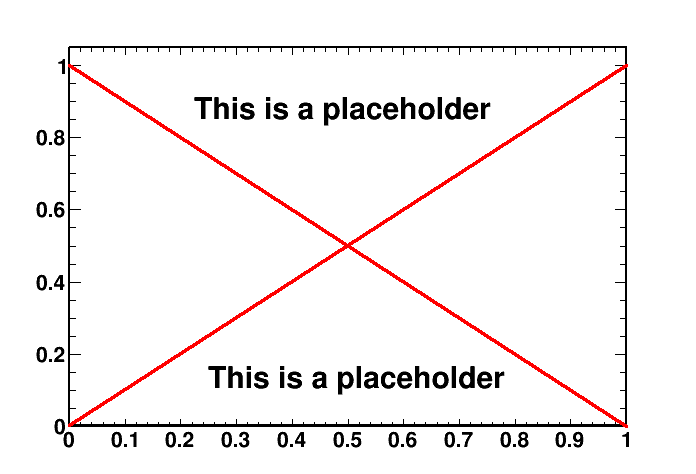
\includegraphics[width=.9\linewidth]{pic/dummy.png}
  \caption{Picture of GC excess, (compare with previous papers?), a chi2 map too}
  \label{fig:original_GC_excess}
\end{figure}

Before trying upgrade the model in use, it is i;portant to make sure we can recreate it in with the same parameters. Fig. \ref{fig:original_GC_excess} shows the results of a fit using only the PCR, IC and BR components. The shape and intensity of the previously observed excess \todo{cite} are found.\\

\begin{figure}
  \centering
  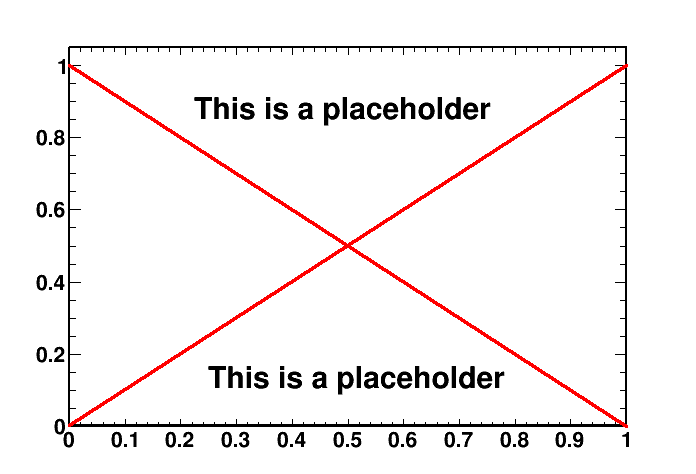
\includegraphics[width=.9\linewidth]{pic/dummy.png}
  \caption{Picture background only spectra with bad fit (high energies too hard) Compare bubble or disk region and outside}
  \label{fig:bkgd_only_spectrum}
\end{figure}

It can also be observed that the fit is particularly bad in the bubbles and the disk (see Fig. \ref{fig:original_GC_excess}) where the high energy spectrum harder (see Fig. \ref{fig:bkgd_only_spectrum}). In this region, the PCR spectrum falls off too quickly, and the IC spectrum which usually takes care of high energies is blocked by the low energy flux drop.


%I was able to recreate a more or less spherical excess in GC around 2GeV.\\
%Bad fit in disk and bubbles as expected.
%Two problems :
%\begin{itemize}
%\item Spectrum too hard at high energies
%\item Excess around 2GeV
%\end{itemize}


\section{Introducing SCR}

\begin{figure}
  \centering
  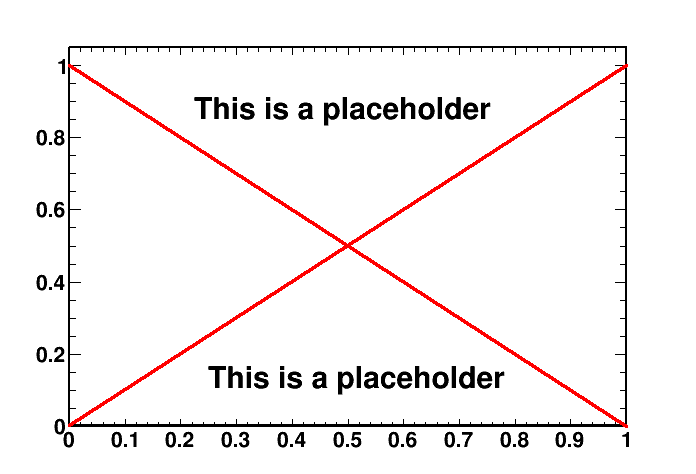
\includegraphics[width=.9\linewidth]{pic/dummy.png}
  \caption{Chi2 maps of SCRonly fits. Spectrum from a bubble.}
  \label{fig:SCRonly_fit}
\end{figure}

Introducing the SCR template, a clear improvement can be noted in the bubbles. The high energy structures are fitted by the new template and the chi2 map does not show the bubbles anymore.

A problem remains for the disk and diffuse regions near the galactic anticenter.



\section{Introducing SCR and MCR}
%	-Introduction of SCR and MCR
%		-very good chi2 in disk and bubbles
%		-spatial shapes of comps
%			-IC sperical (as expected) but depletion in disk
%			-BR low in bubbles replaces IC in disk
%			-PCR OK but low in disk
%			-MCR follows CO map, take place of PCR in disk
%			-SCR follows bubble structure

\begin{figure}
  \centering
  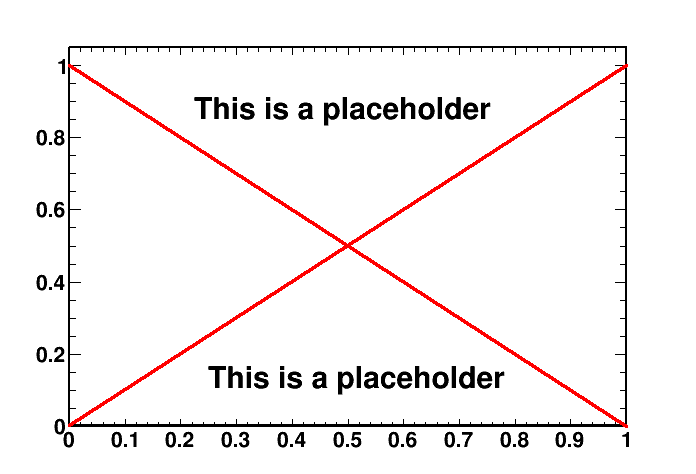
\includegraphics[width=.9\linewidth]{pic/dummy.png}
  \caption{Chi2 maps of MCRonly fits compared to background only}
  \label{fig:MCRonly_fit}
\end{figure}
%First obvious thing is the good chi2 in the disk and bubbles.\\

Adding an other template on top of SCR, the fit can significantly improve in every directions. The shape of the bubbles and the disk are fitted with $chi^2$ close to 1. 


\subsection{Discussion on spatial shapes}
\begin{figure}
  \centering
  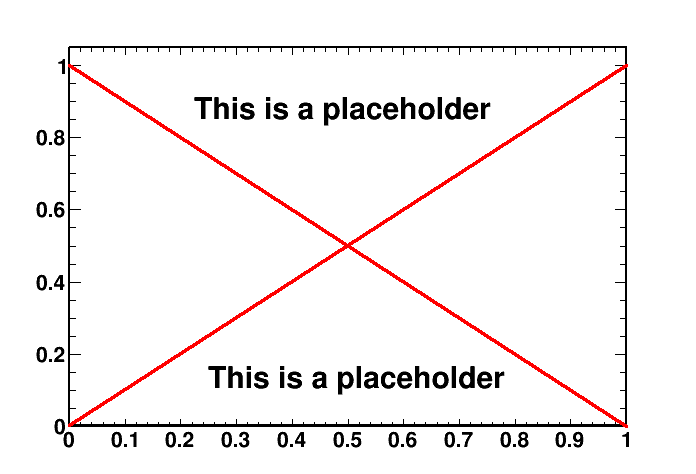
\includegraphics[width=.9\linewidth]{pic/dummy.png}
  \caption{pictures of each component's spatial distributions. Maybe on a full page.}
  \label{fig:spatial_shapes}
\end{figure}
IC is more or less spherical as expected (starlight). There is a disturbing sandwich structure!
BR is consitent with what is expected.
PCR looks OK too, but has the same sandwich structure as IC. Maybe MCR takes too much space in the disk, or proton spectrum is not perfectly correct.
MCR follows very well a gas map (traced by CO).
SCR draws almost perfectly the disk and bubbles as expected.


\section{Introducing SCR and DM}
%	-Introduction of SCR + DM
%		-chi2
%		-spatial shapes	
%		-Weniger plots
%		-Specklings

\begin{figure}
  \centering
  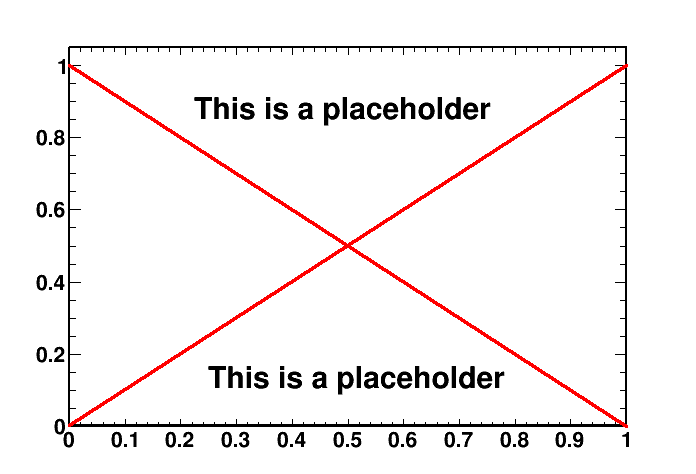
\includegraphics[width=.9\linewidth]{pic/dummy.png}
  \caption{spectrum of best mass DM fitted in CMZ. Also pictures of DM distribution compared to gas map.}
  \label{fig:DMonly_fit}
\end{figure}

Determination of best WIMP mass around 50GeV in CMZ.
DM shape follows the gas map too (like MCR). That does not make any sense.



\section{Introducing SCR and MSP}
%	-Introduction of SCR + MSP:
%		-chi2
%		-spatial shapes
%		-Weniger plots
%		-Specklings

\begin{figure}
  \centering
  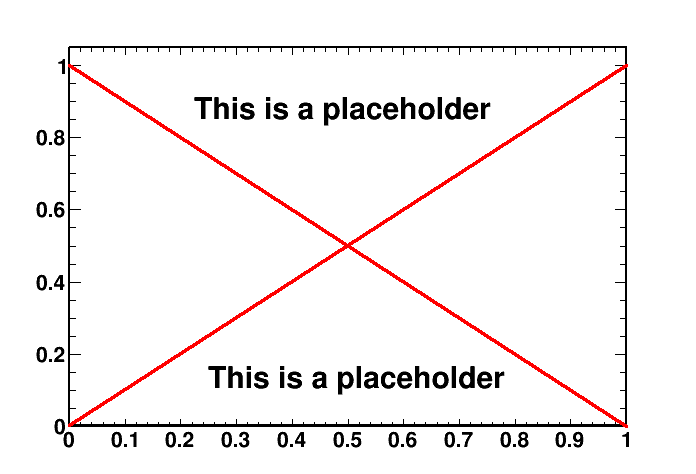
\includegraphics[width=.9\linewidth]{pic/dummy.png}
  \caption{pictures of MSP spectrum, chi2. Residuals at low energy maybe?}
  \label{fig:MSPonly_fit}
\end{figure}

Bad chi2 compared to MCR. The low energy spectrum is too hard.






